%!TEX root = main.tex
\afterpage{\blankpage}
\newpage
\chapter{StackLetter -- personalizovaný informačný bulletin pre Stack Exchange}

\textit{StackLetter} je systém pre vytváranie a rozosielanie personalizovaných informačných bulletinov v rámci platformy
Stack Exchange. Tento systém vznikol ako súčasť spolupráce autora tejto práce a Bc. Matúša Saláta~\cite{Salat2018} v rámci
dvoch diplomových prác riešených v akademickom roku 2016/17 a 2017/18. Celý systém sa skladá
z viacerých spolupracujúcich modulov, ktoré však boli vyvíjané samostatne a sú od seba navzájom nezávislé. Rozdelenie
systému na nezávislé moduly umožňuje rýchlejší vývoj, ako aj možnosť jednoduchého rozširovania systému v budúcnosti.
Architektonický prehľad celého systému znázorňuje obrázok~\ref{fig:architecutre-overview}. Ďalej v tejto práci opisujem
len mnou navrhnuté moduly.

\begin{figure}[H]\begin{center}
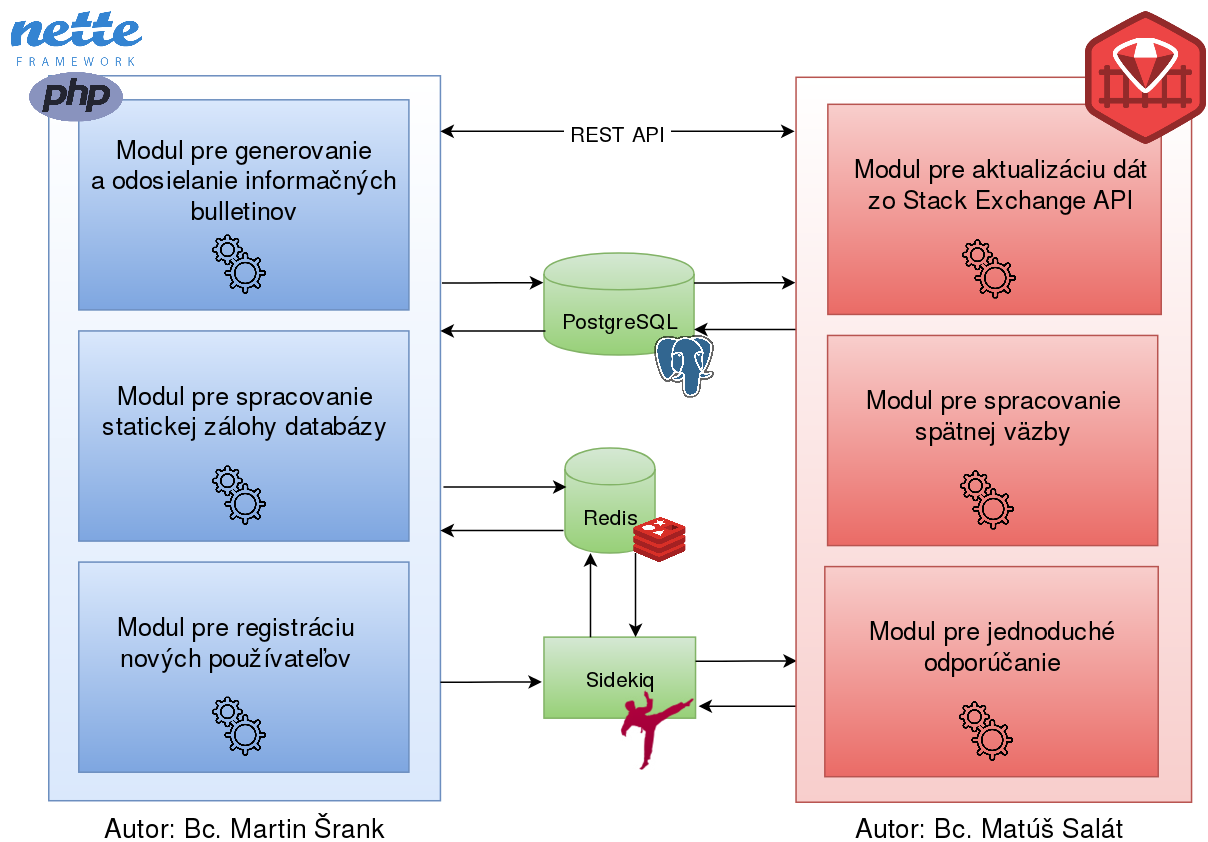
\includegraphics[scale=0.32]{architecture-overview}
\caption{Architektonický prehľad systému StackLetter. \label{fig:architecutre-overview}}\end{center}
\end{figure}

\section{Prehľad modulov}

\textbf{Modul pre registráciu nových používateľov}\\
Tento modul predstavuje používateľmi viditeľnú časť systému. Prostredníctvom webovej stránky systému
-- \url{www.stackletter.com} -- sa používatelia môžu prihlásiť k odoberaniu informačného bulletinu pre niektoré
z ponúkaných komunít platformy Stack Exchange, ako aj spravovať svoje nastavenia týkajúce sa odosielania informačných
bulletinov.\\
Používatelia sa prihlasujú prostredníctvom svojho Stack Exchange konta využitím protokolu OAuth.

\begin{figure}[H]\begin{center}
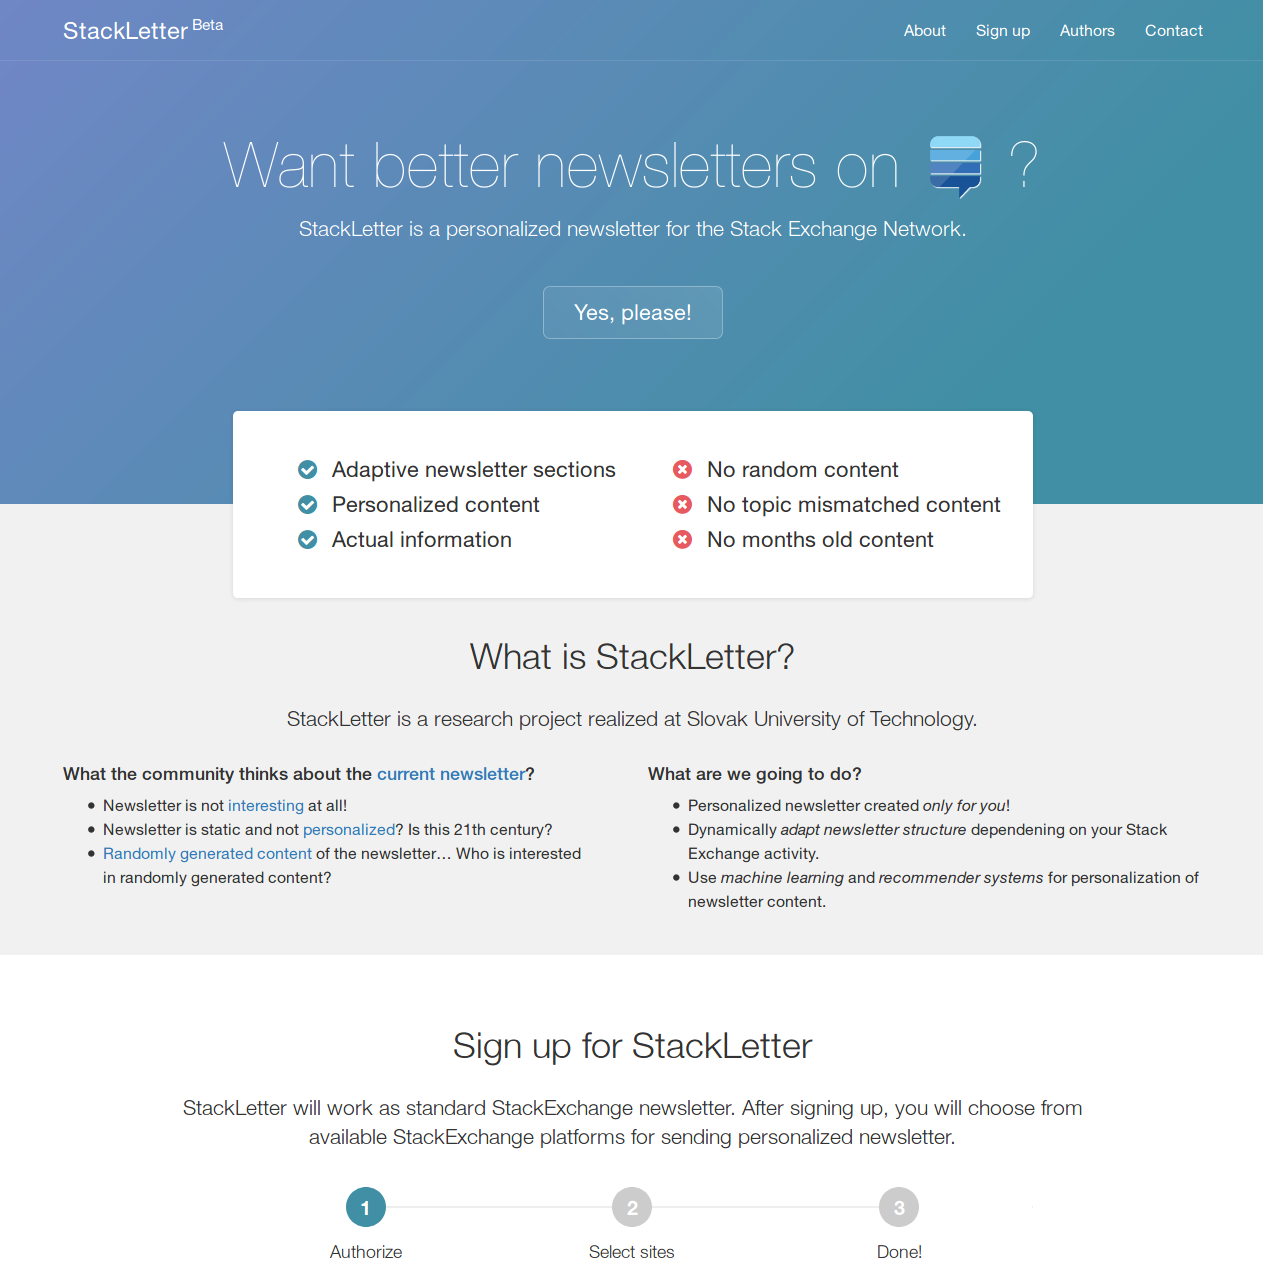
\includegraphics[scale=0.35]{stackletter-screenshot}
\caption{Snímka registračnej stránky StackLetter.com. \label{fig:stackletter.com}}\end{center}
\end{figure}

\textbf{Modul pre generovanie a odosielanie informačných bulletinov}\\
Tento modul je zodpovedný za samotné zostavovanie a odosielanie informačných bulletinov jednotlivým zaregistrovaným
používateľom. Prostredníctvom REST API komunikuje s modulmi pre zostavovanie odporúčaní a štruktúry informačných bulletinov
a na základe ich odpovedí vygeneruje naformátované informačné bulletiny, ktoré sú následne rozosielané prostredníctvom služby
SendGrid\footnote{\url{https://sendgrid.com}}.

\textbf{Modul pre spracovanie statickej zálohy databázy}\\
Modul bol navrhnutý a implementovaný za účelom rýchleho a efektívneho importovania počiatočných dát platformy Stack Exchange
dostupných vo forme XML exportu do našej internej reprezentácie v databáze PostgreSQL.

\textbf{Modul pre personalizované odporúčanie}\\
Modul zabezpečuje samotné vytváranie personalizovaných zoznamov odporúčaní prostredníctvom metódy navrhnutej v tejto práci.
Podrobne sa realizácii tohto modulu venujeme v kapitole~\ref{impl:rec}.

Podrobný technický a architektonický popis jednotlivých modulov sa nachádza
v prílohe~\ref{tech-doc} -- \textit{Technická dokumentácia systému StackLetter}.

\section{Použité technológie a služby}

\begin{my_itemize}
\item{Jednotlivé moduly zabezpečujúce infraštruktúru systému StackLetter sú implementované v~jazyku PHP\footnote{\url{https://php.net}}
verzie~7.1 s použitím MVC frameworku Nette~2.4\footnote{\url{https://nette.org}}.}
\item{Systém na ukladanie dát využíva relačný databázový systém PostgreSQL vo verzii 9.6 a~vnútropamäťové dátové úložisko Redis
vo verzii 4.0.}
\item{Systém komunikuje s platformou Stack Exchange prostredníctvom Stack Exchange API v2.2 a~vykonáva autentifikáciu
používateľov prostredníctvom protokolu OAuth 2.0.}
\item{Na hromadné odosielanie informačných bulletinov používateľom prostredníctovm e-mailu je využitá služba SendGrid.}
\item{Modul pre zostavovanie personalizovaných informačných bulletinov so zameraním na diverzitu je implementovaný
v jazyku Python 3.6 s použitím knižníc scikit-learn, numpy (pre prácu s modelmi) a Flask (pre implementáciu REST API).}
\end{my_itemize}


\section{Realizácia personalizovaného odporúčania}
\label{impl:rec}

Modul pre personalizované odporúčanie je navrhnutý ako samostatný modul, ktorý poskytuje REST API pre komunikáciu
s modulom pre generovanie a odosielanie informačných bulletinov. Vďaka tomu je možné do budúcnosti jednoducho nahradiť
tento modul iným modulom bez potreby výrazných zásahov do existujúcich častí systému.

Každý informačný bulletin sa skladá z troch sekcií, ktoré sú vyberané personalizovane pre jednotlivých používateľov.
Zoznam všetkých dostupných sekcií a aj výber sekcií pre konkrétneho používateľa je témou práce spolužiaka Matúša Saláta\cite{Salat2018},
preto sa mu v tejto práci nevenujeme.

\subsection{Zostavenie LDA a TF-IDF modelov}

\textbf{Slovník}\\
Pre LDA a TF-IDF modely využívané v navrhnutej metóde sme vytvorili slovnú zásobu pozostávajúcu z 500 tisíc náhodne vybraných
otázok z komunity Stack Overflow. Texty prešli predspracovaním v podobe odstránenia formátovania (HTML tagov), diakritiky,
anglických stop slov a lematizáciou. Minimálna dokumentová frekvencia bola stanovená na $5$ a maximálna dokumentová frekvencia na $99\%$.
Okrem toho bola maximálna veľkosť slovníka stanovená na 150 tisíc výrazov, pričom skutočný počet výrazov bol cca 152 tisíc.
Na vytvorenie slovníku bol použitý \textit{CountVectorizer} z~knižnice \textit{scikit-learn}.

\textbf{Nastavenie a trénovanie LDA modelu}\\
Pravdepodobne najdôležitejším parametrom pri latentnej Dirichletovej alokácii je určenie počtu LDA tém. Pre určenie počtu sme
na testovacie dáta (náhodne vybraných stotisíc otázok) opakovane aplikovali zhlukovanie prostredníctvom metódy K-Means, pričom
hodnotu $k$ (počet zhlukov) sme vyberali z intervalu $<20,100>$. Pre každú hodnotu $k$ sme následne vypočítali priemerný siluetový koeficient
(viď.~Obr.~\ref{fig:silhouette}). Na základe tejto analýzy sme stanovili počet LDA tém na 50.

\begin{figure}[H]\begin{center}
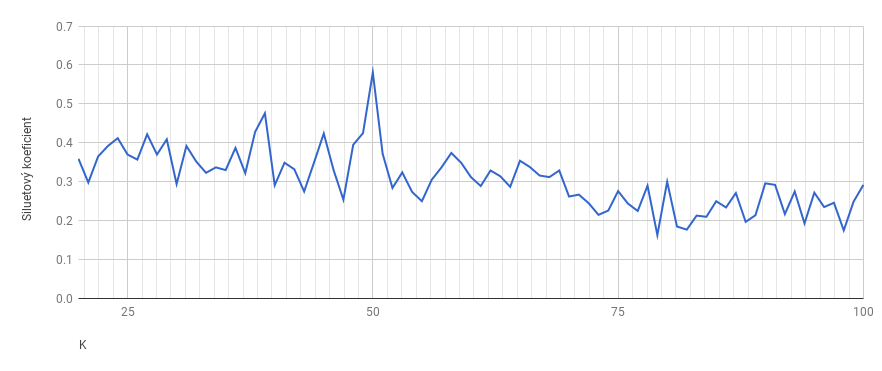
\includegraphics[scale=0.53]{silhouette}
\caption{Siluetový koeficient vzhľadom na $K$ -- počet zhlukov. \label{fig:silhouette}}\end{center}
\end{figure}

LDA model sme natrénovali na vzorke stotisíc náhodne zvolených otázok zo Stack Overflow, pričom sme využili slovník výrazov
vytvorený v predošlom kroku. Ostatné parametre modelu boli nastavené tak, ako boli definované v kapitole~\ref{design:lda-setup}.
Bola použitá implementácia LDA z~knižnice \textit{scikit-learn}.

\textbf{TF-IDF model}\\
TF-IDF model zostavujeme zvlášť pre každého používateľa z otázok, s ktorými interagoval, a to pri každom pretrénovaní používateľských
profilov, ktoré sa vykonáva raz denne pre používateľov s denným informačným bulletinom a raz týždenne pre používateľov s týždenným
bulletinom. Využíva sa implementácia \textit{TfidfTransformer} z~knižnice \textit{scikit-learn}.


\subsection{Vytváranie profilov otázok a používateľov}

\textbf{Profil otázky}\\
Profil otázky sa skladá z troch vektorov: 1) vektor značiek (tagov), ktorými je otázka označená, 2) vektor reprezentujúci
distribúciu otázky v rámci LDA tém a 3) TF vektor. Vektor značiek sa vytvára za behu priamo požiadavkou do databázy. TF vektor
sa tiež vytvára až za behu z textu otázky, nakoľko sa jedná o veľmi rýchlu operáciu. Vektor distribúcie LDA tém sa vytvára
vždy pri vzniku novej otázky, alebo po interakcii používateľa s otázkou, pre ktorú ešte nebol vytvorený. Tento vektor
sa po vytvorení ukladá do databázy. Vytváranie profilov pre novo vzniknuté otázky sa vykonáva raz denne.

\textbf{Profil používateľa}\\
Profil používateľa sa nevytvára za behu, ale sa perzistuje v binarizovanej podobe do súboru, odkiaľ sa v prípade použitia
načítava. Profil používateľa sa delí na podprofily záujmu a expertízy, pričom tie sa vytvárajú z profilov otázok, s ktorými
používateľ interagoval.

Každý podprofil sa skladá z vektoru značiek, ktorý predstavuje relatívne zastúpenie značiek v otázkach, s ktorými používateľ interagoval,
normalizovaných do intervalu $<0,1>$; vektoru LDA tém, ktorý je vytvorený analogicky a tiež normalizovaný do intervalu $<0,1>$,
a matice TF vektorov z profilov príslušných otázok. Z tejto matice sa následne predpočíta aj matica TF-IDF.

\textbf{Aktualizácia profilov používateľov}\\
Profil používateľa sa aktualizuje v pravidelných intervaloch na základe jeho preferencie prijímania informačných bulletinov, teda
denne alebo týždenne. Pre zachytenie meniacich sa záujmov používateľa v čase (viď kapitola~\ref{design:freshness}) sa využíva
exponenciálny faktor úpadku: $df = (1-d)^t$.

Čas ($t$) sa udáva ako počet aktualizácií profilu, a percentuálny pokles ($d$)
sa vypočíta ako podiel množstva používateľovej aktivity od poslednej aktualizácie profilu a celkového množstva používateľovej aktivity.
Množstvo používateľovej aktivity sa počíta s príslušnými váhami za jednotlivé aktivity (viď kapitola~\ref{design:userprofile}).
Faktor úpadku sa počíta zvlášť pre oba používateľské podprofily.

Pri aktualizácii profilu používateľa sa najprv týmto faktorom úpadku prenásobia vektory reprezentujúce doterajšiu aktivitu
a následne sa k nim prirátajú hodnoty z obdobia od poslednej aktualizácie. Vektory značiek a LDA tém sa následne nanovo
normalizujú a z TF matice sa nanovo predpočíta matica TF-IDF.

\textbf{Použitie podprofilov používateľov v sekciách informačného bulletinu}\\
Na základe sekcie informačného bulletinu, pre ktorú sa vytvára zoznam odporúčaní sa využíva buď záujmový alebo
expertízny podprofil používateľa, alebo oba, ako popisuje tabuľka~\ref{tab:sections}.

\begin{table}[h]
\label{tab:sections}
\centering
\caption{Sekcie informačného bulletinu a k nim prislúchajúce podprofily používateľa}
\begin{tabular}{|m{7cm}|>{\centering\arraybackslash}m{2.5cm}|>{\centering\arraybackslash}m{2.6cm}|}
\hline
\textbf{Sekcia} & \textbf{Záujmový podprofil} & \textbf{Expertízny podprofil} \\\hline
Najnovšie otázky               & ×  & -- \\\hline
Užitočné otázky                & ×  & -- \\\hline
Otázky čakajúce na odpoveď     & -- & ×  \\\hline
Populárne nezodpovedané otázky & -- & ×  \\\hline
Vysoko diskutované otázky      & ×  & ×  \\\hline
Vysoko diskutované odpovede    & ×  & ×  \\\hline
Zaujímavé odpovede             & ×  & ×  \\\hline
\end{tabular}
\end{table}

\textbf{Komunitný profil používateľov}\\
V prípade, že používateľský profil neobsahuje dostatočné množstvo aktivity pre zostavenie relevantných odporúčaní,
sa použije tzv. \textit{Komunitný profil používateľov}. Ten je presne analogický so štandardným profilom používateľa,
no skladá sa nie z aktivity konkrétneho používateľa, ale zo všetkých položených otázok a odpovedí v celom CQA systéme.
Rovnako ako štandardné používateľské profily sa aj komunitný profil aktualizuje denne a s aplikáciou faktoru úpadku.


\subsection{Zostavenie zoznamu odporúčaní}

Modul pre personalizované odporúčanie podporuje dve metódy pre zostavenie zoznamu odporúčaní -- štandardné personalizované
odporúčanie a personalizované odporúčanie s diverzifikačnou metódou tématického vzorkovania. Tieto dve metódy sme využili
pri overení našich hypotéz prostredníctvom A/B testu (viď kapitola~\ref{sec:experiment}).

\textbf{Personalizované odporúčanie}\label{impl:pers-method}\\
Pri personalizovanom odporúčaní $n$ položiek je proces pomerne priamočiary: na základe sekcie informačného bulletinu
sa vyberie príslušný podprofil používateľa, z ktorého sa následne vyberie $n$ najrelevantnejších značiek
a $\left\lceil\frac{n}{2}\right\rceil$ najrelevantnejších LDA tém. Potom sa z databázy vyberú všetky otázky, položené
od odoslania predošlého informačného bulletinu, ktoré patria do týchto LDA tém alebo značiek.

Prostredníctvom skalárneho súčinu nad TF-IDF maticou vybraných otázok a maticou z profilu používateľa sa potom vytvorí
usporiadaný zoznam otázok, z ktorých je prvých $n$ prezentovaných používateľovi.

\textbf{Personalizované odporúčanie s diverzifikačnou metódou tématického vzorkovania}\\
Podobne ako pri štandardnom personalizovanom odporúčaní sa najprv vyberie určitá množina značiek a LDA tém z
príslušného používateľského podprofilu. Pre každú z nich sa následne rovnakou metódou zostaví zoznam odporúčaní.
Tieto jednotlivé zoznamy sa potom spoja do jedného výsledného zoznamu $n$ odporúčaní. Podrobnosti metódy tématického
vzorkovania sú uvedené v kapitole~\ref{sec:thematic-sampling}.

V prípade, že metóda odporúčania s diverzifikáciou nevráti dostatočne početný zoznam odporúčaní, doplní sa zoznam
o položky získané z metódy personalizovaného odporúčania. Tento prípad môže nastať hlavne v prípade denného informačného
bulletinu, ak sa vyberú značky s veľmi malým počtom nových otázok.

Obe metódy tiež zabezpečujú, aby používateľovi neboli v jednom informačnom bulletine prezentované tie isté otázky
viackrát.


\section{Charakteristika dát}

Našu prácu sme sa rozhodli realizovať nad dátami z komunity \textit{Stack Overflow},
nakoľko je táto komunita zameraná na doménu, v ktorej máme hlbšie vedomosti a teda vieme lepšie posúdiť správnosť
odporúčania v tejto doméne. Navrhnuté riešenie však nie je špecifické pre túto komunitu a je možné ho nasadiť v rámci
celej platformy Stack Exchange, prípadne na iných CQA systémoch s podobnou štruktúrou.

Komunita Stack Overflow, ktorej dáta sme použili, je jednoznačne najväčšou a najaktívnejšou zo všetkých komunít
platformy Stack Exchange a má nasledovný rozsah \emph{(údaje sú zaokrúhlené)}:

\begin{my_itemize}
    \item{Otázky -- 16 miliónov}
    \item{Odpovede -- 24 miliónov}
    \item{Používatelia -- 9 milíonov}
    \item{Komentáre -- 66 milíonov}
    \item{Značky -- 52 tisíc}
    \item{Priemerný denný prírastok otázok -- 7 tisíc}
    \item{Priemerný denný prírastok odpovedí -- 7.5 tisíc}
    \item{Priemerný denný prírastok komentárov -- 26 tisíc}
\end{my_itemize}

\textbf{Archívne dáta}\\
Platforma Stack Exchange zverejňuje archív všetkých komunít vo forme XML výstupov. Dáta v tomto
archíve\footnote{\url{http://archive.org/details/stackexchange}} sú pravidelne aktualizované a obsahujú kompletné
používateľmi vytvorené anonymizované dáta zo všetkých komunít platformy. Všetky tieto dáta sú verejne dostupné pod
licenciou \emph{Creative Commons Attribution-ShareAlike 3.0 Unported}.

Tieto dáta sme využili v prvotnej fáze na vytvorenie základných modelov. Následne sa využívali dáta získané
prostedníctvom verejného API poskytovaného platformou Stack Exchange.

Štruktúra dát v archívoch je nasledovná:

\begin{my_itemize}
  \item{\textit{Badges.xml} -- Obsahuje ID používateľov, názvy odznakov a čas, kedy používateľ odznak získal.}
  \item{\textit{Comments.xml} -- Obsahuje všetky komentáre spolu s informáciou o ich autoroch a príspevkoch, ku ktorým sa viažu.}
  \item{\textit{Posts.xml} -- Obsahuje informácie o všetkých príspevkoch (otázkach a odpovediach) a k nim prislúchajúce značky, ako aj aktuálne znenie príspevku}
  \item{\textit{PostHistory.xml} -- Obsahuje históriu zmien jednotlivých príspevkov, ako napr. zmenu názvu, štítkov, označenie otázky za zodpovedanú a pod.}
  \item{\textit{Users.xml} -- Obsahuje verejné údajé všetkých používateľov, ako sú meno, reputácia, webová stránka, počet hlasov a iné.}
  \item{\textit{Votes.xml} -- Obsahuje anonymizované informácie o hlasoch príspevkov.}
\end{my_itemize}

Dátový archív komunity Stack Overflow poskytuje všetok obsah od vzniku systému (cca 200GB dát vo formáte XML). Nakoľko
však pre naše účely (zostavenie slovníka výrazov, natrénovanie LDA tém) nie je potrebný celý archív,
rozhodli sme sa použiť len obmedzené množstvo archívnych dát, konkrétne len príspevky od 1.6.2017.
Okrem nich boli tiež stiahnuté všetky príspevky, s ktorými v minulosti prišli do kontaktu odoberatelia nášho informačného
bulletinu. Keďže informačné bulletiny majú charakter periodického média s veľkým dôrazom na aktuálnosť obsahu, toto
obmedzenie sa len na určitú podmnožinu dát nemá na výsledky žiaden signifikantný vplyv.
